\section{Experimental Setup}
\label{sec:experimentalSetup}

Our evaluation compares five different continuous sensing methods: 1) always on,
2) duty cycling, 3) sensor data batching, 4) predefined activity detection, and
5) our filter-based approach for specifying custom wakeup conditions. We
implement applications using these different sensing methods and use trace-based
simulation for comparison. The rest of this section describes our trace
collection methodology, the sensing applications that we have implemented, and
the operation of our trace-based simulator.

%%  alternative implementations of
%% applications that perform continuous sensing.  We consider approaches that
%% assume that the phone is always-on, performs duty cycling, has access to
%% hardware that buffers sensor readings, provides an API that either lets
%% applications register for notifications based on pre-defined activity
%% recognition, and provides an API that lets applications specify custom wakeup
%% conditions by configuring pre-defined filters.

\subsection{Trace Collection}

We use traces in our evaluation because they help provide the same
input to the different sensing methods. To compare these methods, we
need ground truth about the occurrence and the timing of desired
events, such as steps taken. Annotating accelerometer traces collected
from human subjects with the ground truth is time-consuming and error
prone.

Instead, we used an AIBO ERA 210 robot dog (see Figure~\ref{fig:aibo})
to collect the ground truth about events and accelerometer traces for
our experiments. The robot performed a sequence of actions in a
course, and we logged these actions and the timestamps for the
beginning and the end of each action. This log represents the ground
truth for our experiments. We also logged the robot's accelerometer
readings by attaching a Google Nexus 4 to the back of the robot.

To get statistically significant results, the robot was programmed to
perform its course multiple times. Each course generated a separate
ground truth log and an accelerometer trace. In a course, the robot
performed five different actions: standing idle, walking,
seat-to-stand transition, stand-to-seat transition, and headbutt. To
eliminate bias, these actions were generated randomly in each
course. We divided courses into three different groups to cover a
range of activity levels. Courses in groups 1, 2 and 3 spent 90\%,
50\% and 10\% of the time standing idle, respectively. The reminder of
the time was allocated as follows: 90\% for walking, 9\% for
transitions between seating and standing, and 1\% for headbutts. This
setups allows us to experiment with detecting actions that are common,
somewhat frequent, and rare. Figure~\ref{fig:actionTimes} shows the
average amount of time that each action is being performed in the
traces in each group, as a percentage of the average trace
length. {\em TODO: mention how many courses from each group we ran}

\begin{figure}[t]
	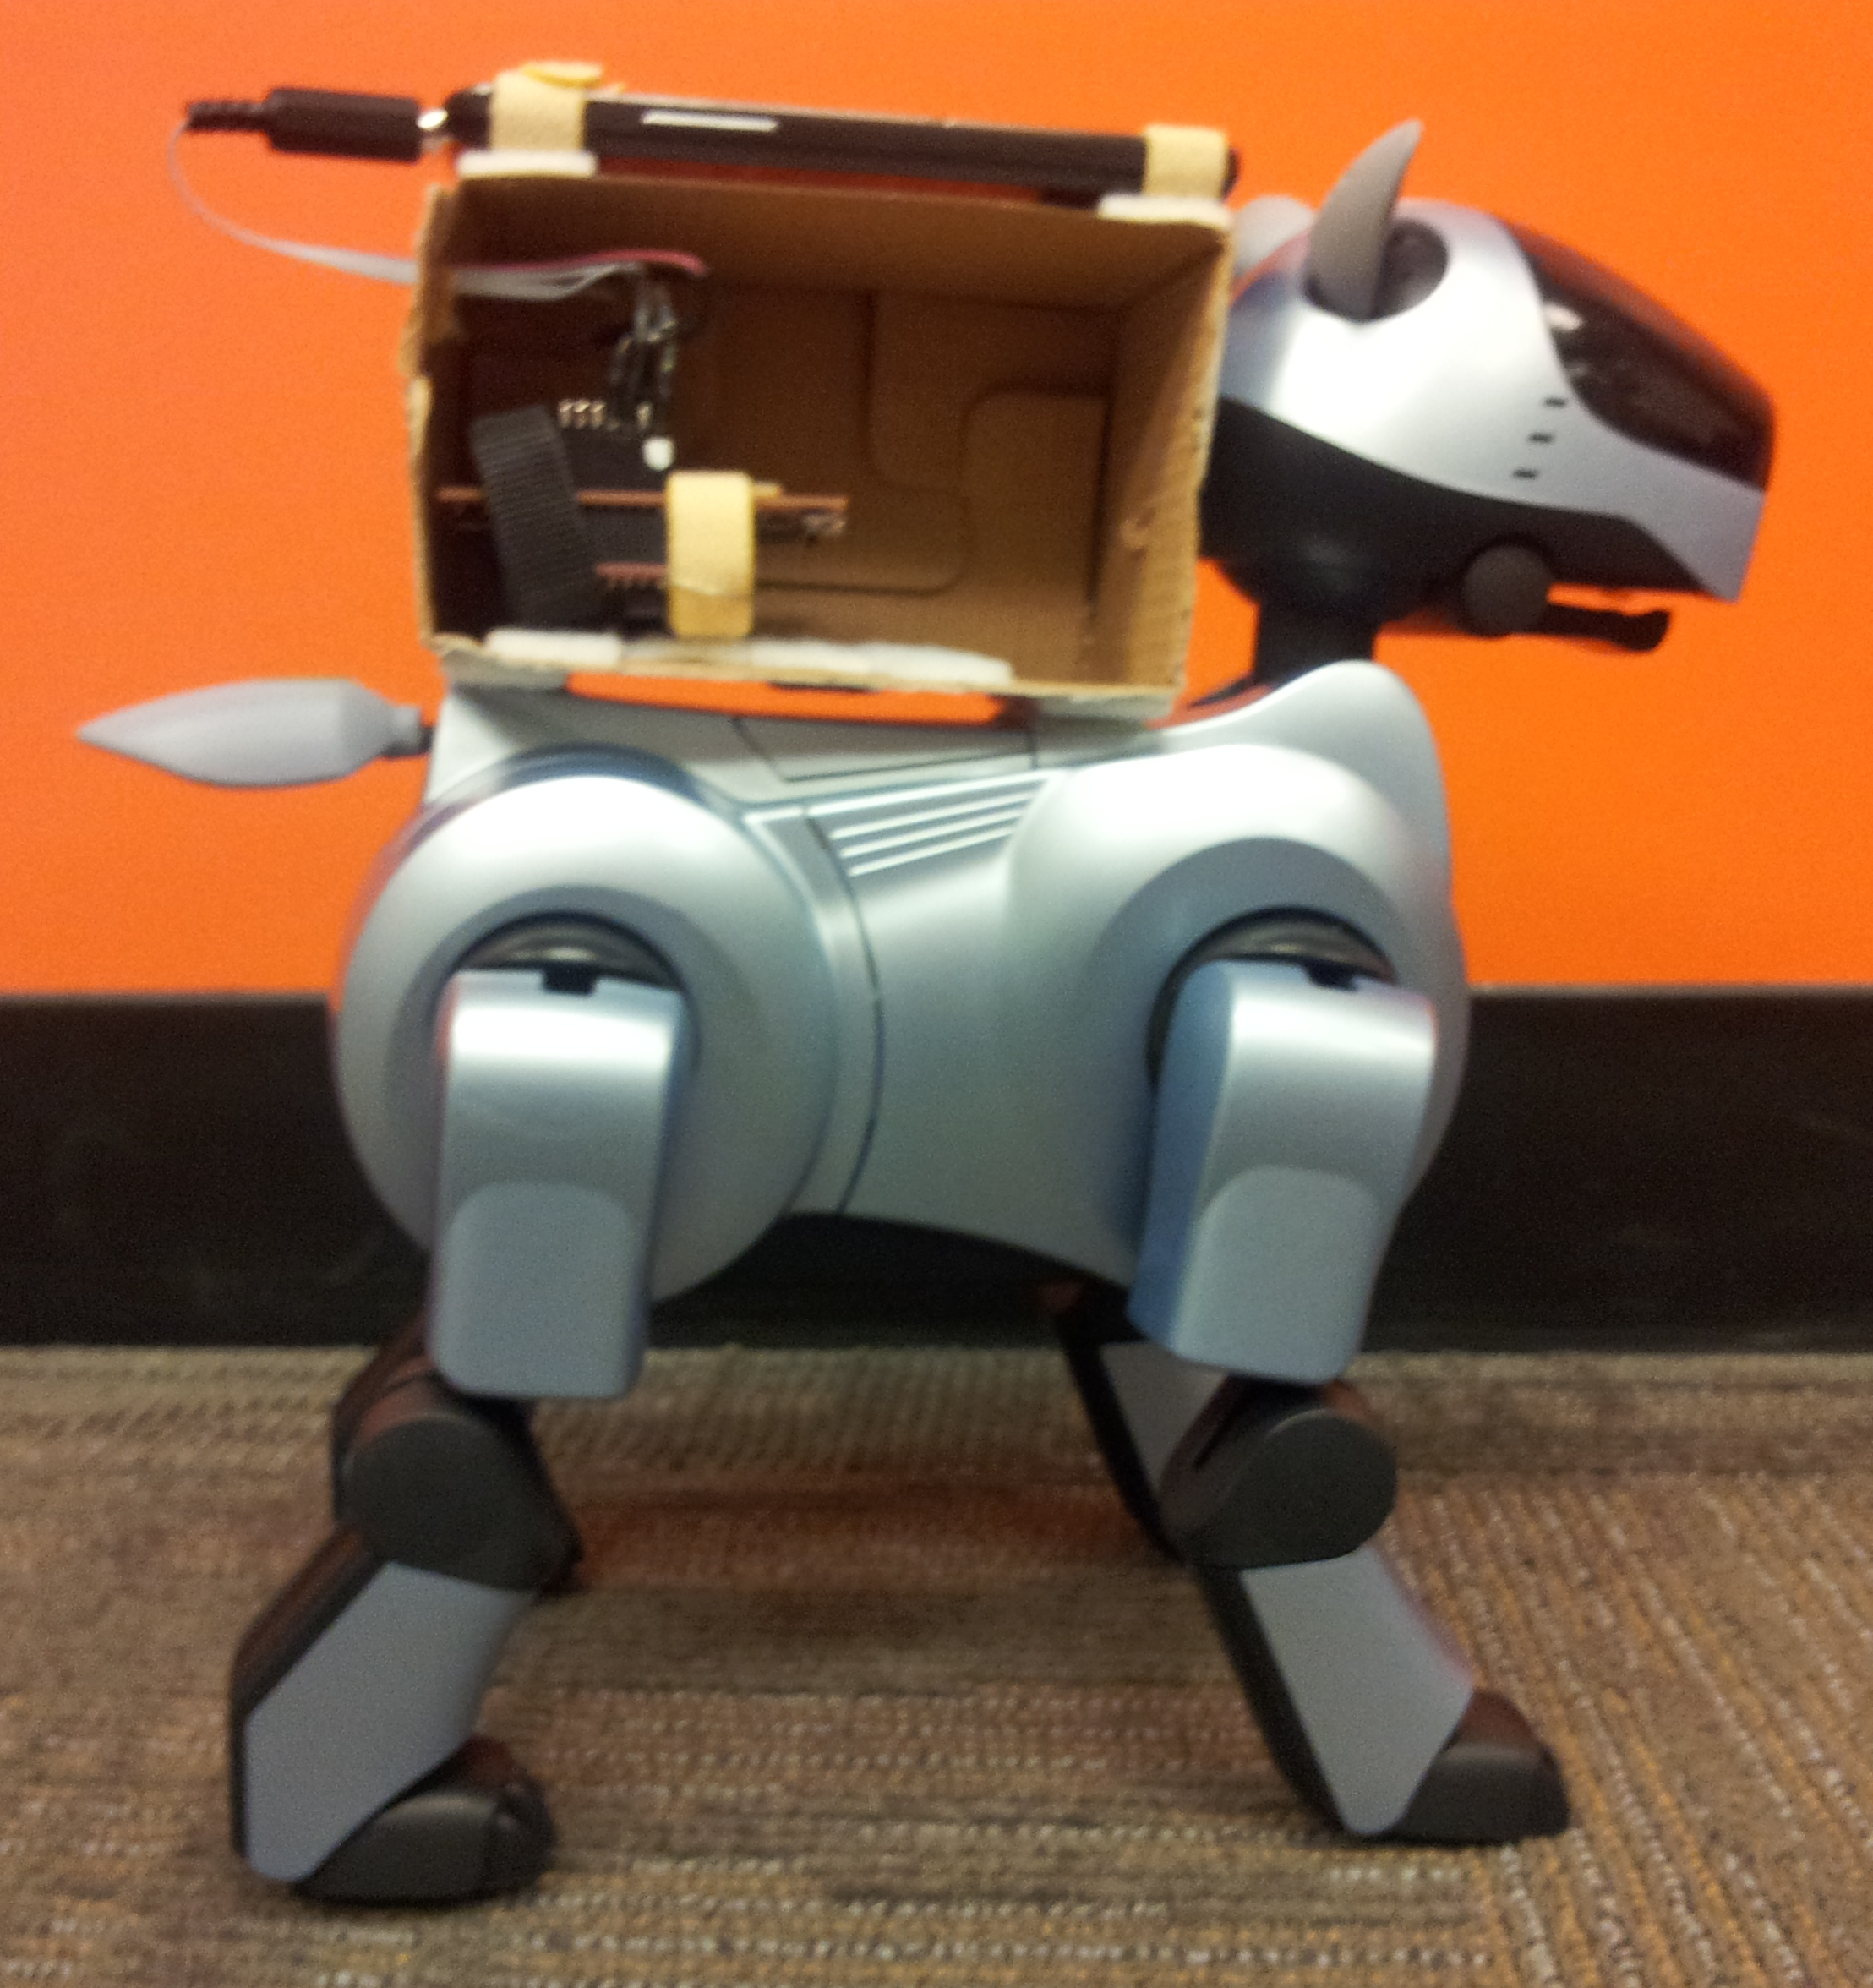
\includegraphics[width=8.5cm]{aibo_ers_210.jpg}
	\caption{AIBO ERS 210 robot used to collect the accelerometer traces}
	\label{fig:aibo}
\end{figure}

\begin{figure}[t]
	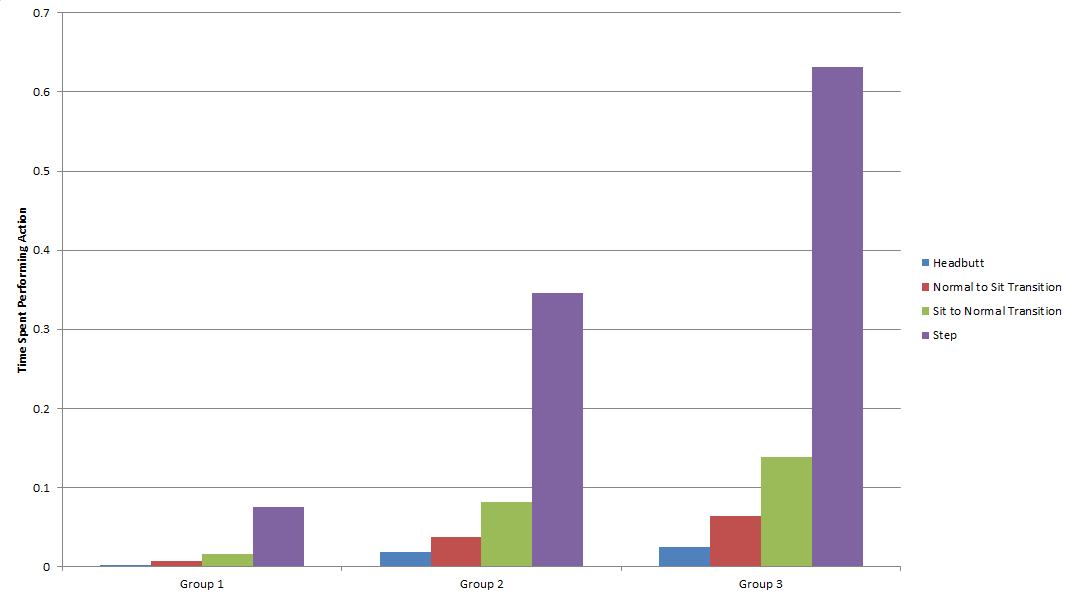
\includegraphics[width=8.5cm]{action_times.png}
	\caption{Time spent performing actions of specific types as a percentage or trace length}
	\label{fig:actionTimes}
\end{figure}

\subsection{Applications}

We have implemented three applications:

\begin{itemize}

\item {\bf Steps} counts how many steps the dog takes when it walks by
  looking for local maxima in the x-axis of the acceleration trace.


\item {\bf Stand-seat} detects transitions between seating and
  standing by monitoring changes in the acceleration due to gravity on
  the y and z axes.

\item {\bf Headbutt} detects a headbutt motion by searching for local
  minima on the y-axis of the acceleration trace.

\end{itemize}

Each application runs a set of low-pass filters based on fast-fourier
transforms (FFT) on the main processor for activity detection. We use
these applications for evaluating always-on operation, duty cycling,
and batching. The activity detection and wake-up condition sensing
methods require programming the low-power processor. To evaluate these
methods, we developed a variant of each application that runs three
types of filters on the low-power processor: 1) simple threshold, 2)
exponential moving average, and 3) FFT. The low power processor wakes
up the phone when these filters indicate that an event of interest has
been detected. The application then runs its FFT algorithms on the
main processor to eliminate false alarms, i.e., events that where
misidentified by the low-power processor.

\subsection{Trace-based Simulator}

The accelerometer trace collected for each course is an ordered set of
accelerometer readings. Each reading contains the x, y and z
components of the acceleration vector and a timestamp indicating when
the reading was produced.

The simulator processes the accelerometer readings one at a time,
similar to the way a mobile device would receive accelerometer
readings in real-time, as they are produced by the sensor. Based on
these readings and the wake-up condition, the simulator determines
when the device would be woken up. The simulator also determines what
readings need to be sent to the running applications. At the end of
the run, the simulator outputs the following metrics:

\textbf{Might be better to put the following text in a table -Ashvin.}

\begin{enumerate}
\setlength{\itemsep}{-3pt}  

\item Amount of time the device would have been awake.

\item Total number of times the device was woken up.

\item Number of times that the device was woken up that did not result
  in an event of interest being detected by the application.

\item True positives, false positives and false negatives for each
  event of interest. \textbf{define each precisely -Ashvin}.

\item Recall and precision for each event of interest. \textbf{define
  each precisely -Ashvin}.

\item Power consumption over the duration of the trace. This value is
  derived from the energy measurements presented in
  Section~\ref{sec:prototype}, the amount of time the device is awake,
  the amount of time it is asleep, and the number of transitions
  between the two states.
\end{enumerate}


\subsection{Discussion}

Since we are mainly interested in actions that would normally be
performed by humans, we configured the robot to perform actions with
similar acceleration signatures. A walking robot has a similar
acceleration signature as its human counterpart, though at a lower
intensity. The headbutts are meant to represent very infrequent human
actions such as falling. We found that robot stance transitions
between the normal and sitting postures are very similar in their
acceleration signature to humans sitting down and standing up.

Rather than using a trace-based simulator, it is possible to run live
experiments with a robot because it can perform a deterministic
sequence of actions multiple times. However, we chose to use the
simulator for several reasons. First, each course takes more than an
hour. Our goal was to obtain results for the various sensing
approaches, and perform an exhaustive exploration of the parameter
configuration space. The combination of multiple courses, wake-up and
parameter configurations would have required over a year of continuous
live experimentation. Moreover, taking fine grain power consumption
measurements while the robot is in motion is not trivial.
Nonetheless, we plan to validate our simulation results using live
experimentation in the future.

\textbf{I think the following text should go in the results section. -Ashvin}

Additionally, the Always Awake simulations show
the accuracy of the implemented applications in terms of event of
interest detection precision and recall. 


Figure \ref{fig:aaRecallByGroup} shows the average recall for all
applications when executing on a phone that is kept always-on.  With
the exception of the headbutt action in Group 1, event recall is above
95\% for all actions and groups. The headbutt action in Group 1
appears to be an outlier because Group 1 contains traces with the
least amount of actions and headbutts are the scarcest actions,
occurring only about once per trace. Figure
\ref{fig:aaPrecisionByGroup2} shows the detection precision of each of
the events of interest averaged over the traces in each group. For all
cases, the applications achieved a detection precision above 82\%.



\begin{figure}[t]
	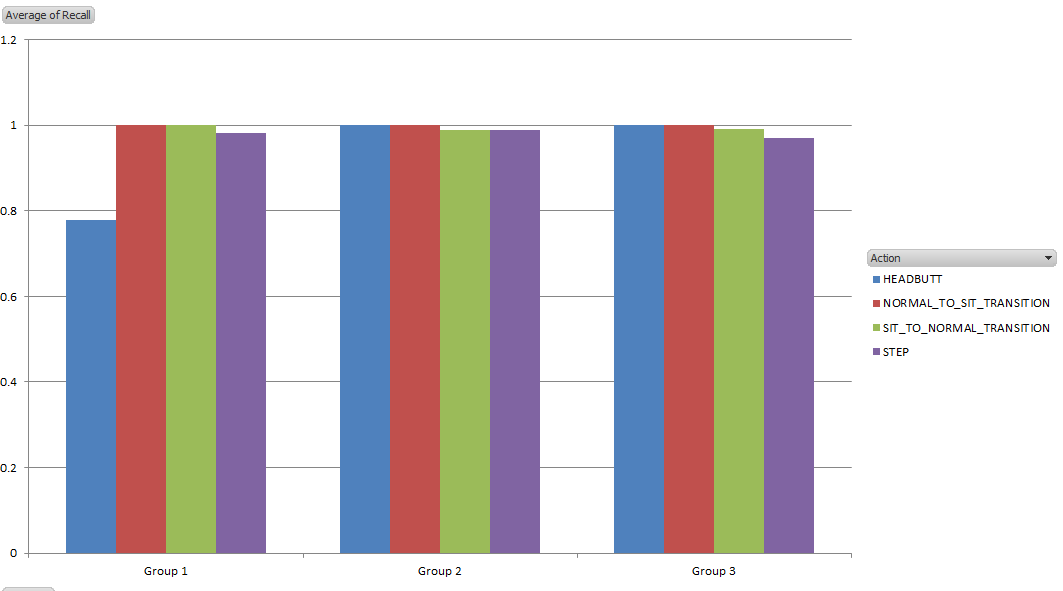
\includegraphics[width=8.5cm]{aa_recall_by_group.png}
	\caption{Always Awake: Recall by Group}
    	\label{fig:aaRecallByGroup}
\end{figure}


\begin{figure}[t]
	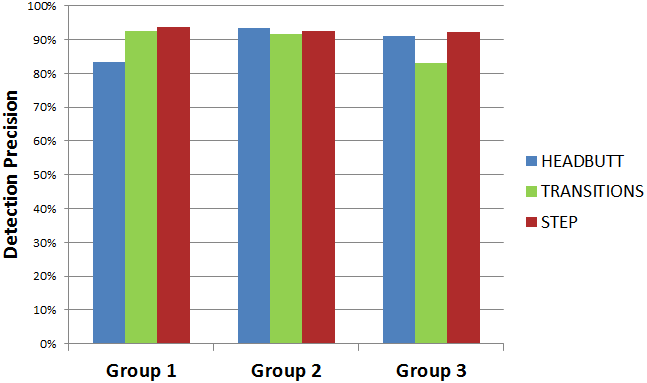
\includegraphics[width=8.5cm]{aa_precision_by_group.png}
	\caption{Always Awake: Detection Precision by Group}
    	\label{fig:aaPrecisionByGroup}
\end{figure}


